
    \section{总结与展望}
    %添加一个目录
    \frame{
     \frametitle{目录}
     \tableofcontents[current,currentsection,sections={<1-5>}]
     \addtocounter{framenumber}{-1}  %目录页不计算页码
    }

    \frame{
      \frametitle{\secname}
      \vspace{-0.5em}
      \begin{block}{总结}
        \footnotesize
        \begin{enumerate}[(1)]
          \item 夯实了基础知识
          \item 完成了论文初稿
          \item 完成了一篇专利初稿,并有了下一篇的思路
          \item 辅助李波老师完成了暑期莫航课堂的学习
        \end{enumerate}
      \end{block}
      \vspace{-0.5em}
      \begin{block}{展望}
        \footnotesize
      \begin{enumerate}[(1)]
          \item 完成论文
          \item 完成专利
        \end{enumerate}
      \end{block}
      
      \note{
        总结一下~\ldots PPT
      }
    }

    % \section{主要参考文献}
    % \frame[t,allowframebreaks]{
    %   \frametitle{\secname}
    % \printbibliography
    % }
    
    % \section{感谢}
    % \frame{
    %   \frametitle{\secname}
    %   \begin{block}{致谢}
    %     \begin{enumerate}[(1)]
    %       \item 导师雍俊海老师的精心指导;
    %       \item 施侃乐老师帮助;
    %       \item 研究所各个项目的历练;
    %       \item 王斌老师、陈莉老师的评审及意见,答辩委员会老师聆听和指导。
    %     \end{enumerate}
    %   \end{block}
    % }


    \section{毕业设计创想}
    \frame{
      \frametitle{目录}
      \tableofcontents[current,currentsection,sections={<1-5>}]
      \addtocounter{framenumber}{-1}  %目录页不计算页码
     }
    \frame{
      \frametitle{\secname}
      \vspace{-0.5em}
      \begin{figure}[htb]   
        \center{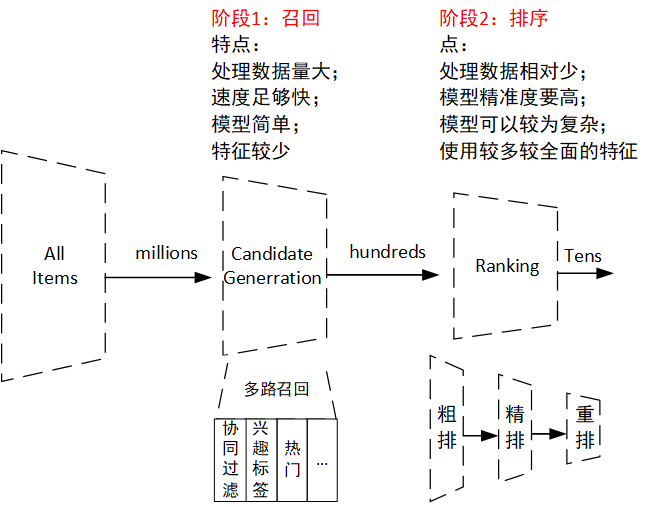
\includegraphics[width=8cm]  {tuijianxitong-liuchengtu.png}}   
        \caption{\label{2} 推荐算法流程}    
      \end{figure}

    }
      \frame{
      \begin{block}{推荐算法 ~\&~  贝叶斯} 
        \footnotesize
        \begin{enumerate}[(1)]
          \item 首先使用常规的推荐算法进行预测
          \item 使用约束参数学习对网络进行学习
          \item 用贝叶斯网络对推荐算法的特征进行精度分析$\xrightarrow{~~ }$降维
          \item 对比网络结果一致性,争取对特征进行解释
          
        \end{enumerate}
      \end{block}
      \vspace{-0.5em}
      \begin{block}{创新点}
        \footnotesize
      \begin{enumerate}[(1)]
          \item 约束参数学习
          \item 贝叶斯网络对推荐算法的特征进行选取,理清其中相关性
        \end{enumerate}
      \end{block}
      
      \note{
        总结一下~\ldots PPT
      }
    }
    \frame{
      \frametitle{ }
      
       ~\\ ~\\
       \center{\Large{Thank you!}}
       \\ ~\\ ~\\ ~\\ ~\\ 

    }